\documentclass[12pt,openany]{book}
\usepackage[a4paper,top=2.5cm,bottom=2.5cm,left=2cm,right=2cm]{geometry}

\usepackage{graphicx}

\usepackage{amsmath}

\usepackage[numbers]{natbib}

\usepackage[breaklinks,hidelinks]{hyperref}

\usepackage{booktabs}

\usepackage{tcolorbox}
\tcbuselibrary{skins}

\usepackage{xcolor}

\usepackage{fancyhdr}
\pagestyle{plain}

% Glossary of mathematical symbols
\usepackage{siunitx}
\sisetup{per-mode = symbol}
\usepackage[symbols,nogroupskip,sort=none]{glossaries-extra}
\glsxtrnewsymbol[description={Control signal for fuel mass flow rate (\si{\kg\per\s}).}]{cm}{\ensuremath{c_{\dot{m}}}}
\glsxtrnewsymbol[description={Control signal for thrust force orientation (radians).}]{ctheta}{\ensuremath{c_{\theta}}}
\glsxtrnewsymbol[description={Total force on the rocket (\si{\N}).}]{F}{\ensuremath{\mathbf{F}}}
\glsxtrnewsymbol[description={Aerodynamic drag force acting on the rocket (\si{\N}).}]{FD}{\ensuremath{\mathbf{F}_D}}
\glsxtrnewsymbol[description={Gravitational force acting on the rocket (\si{\N}).}]{FG}{\ensuremath{\mathbf{F}_G}}
\glsxtrnewsymbol[description={Thrust force (\si{\N}).}]{FT}{\ensuremath{\mathbf{F}_T}}
\glsxtrnewsymbol[description={Magnitude of the thrust force (\si{\N}).}]{FTmag}{\ensuremath{F_T}}
\glsxtrnewsymbol[description={Standard acceleration due to gravity at sea level (constant), $g_0=\num{9.80665}$ (\si{\m\per\s\squared}).}]{g0}{\ensuremath{g_0}}
\glsxtrnewsymbol[description={Specific impulse, $I_{sp}=\gls{ve}/\gls{g0}$ (\si{\s}).}]{Isp}{\ensuremath{I_{sp}}}
\glsxtrnewsymbol[description={Instantaneous mass of the rocket (\si{\kg}).}]{m}{\ensuremath{m}}
\glsxtrnewsymbol[description={Initial mass of the rocket (\si{\kg}).}]{m0}{\ensuremath{m_0}}
\glsxtrnewsymbol[description={Final mass of the rocket (\si{\kg}).}]{mf}{\ensuremath{m_f}}
\glsxtrnewsymbol[description={Time (\si{\s}).}]{t}{\ensuremath{t}}
\glsxtrnewsymbol[description={Final time (\si{\s}).}]{tf}{\ensuremath{t_f}}
\glsxtrnewsymbol[description={Velocity of the rocket (\si{\m\per\s}).}]{v}{\ensuremath{\mathbf{v}}}
\glsxtrnewsymbol[description={Magnitude of the velocity of the rocket (\si{\m\per\s}).}]{vmag}{\ensuremath{v}}
\glsxtrnewsymbol[description={Initial velocity of the rocket (\si{\m\per\s}).}]{v0}{\ensuremath{v_0}}
\glsxtrnewsymbol[description={Average exhaust speed along the engine axis (\si{\m\per\s}).}]{ve}{\ensuremath{v_e}}
\glsxtrnewsymbol[description={Final velocity of the rocket (\si{\m\per\s}).}]{vf}{\ensuremath{v_f}}
\glsxtrnewsymbol[description={Change in rocket velocity for a free burn (\si{\m\per\s}).}]{dv}{\ensuremath{\Delta v}}
\glsxtrnewsymbol[description={Position of the rocket (\si{\m}).}]{x}{\ensuremath{\mathbf{x}}}

\renewcommand{\contentsname}{Table of Contents}

% Paragraph setting
\setlength{\parindent}{0em}
\setlength{\parskip}{1em}

% Set fonts
\usepackage{fontspec}
\setmainfont{Tex Gyre Pagella}
\setsansfont{Verdana}

% Chapter styling
\usepackage[grey]{quotchap}
\makeatletter
\renewcommand*{\chapnumfont}{%
  \usefont{T1}{\@defaultcnfont}{b}{n}\fontsize{80}{100}\selectfont% Default: 100/130
  \color{chaptergrey}%
}
\makeatother
\renewcommand{\bibname}{References}

\title{
  The Haskell Space Program\\
  Planning an Orbital Launch
}
\author{
  Jonathan Merritt
  \and
  Luke Clifton
}
\date{Feb 2019}

\begin{document}
\maketitle
\tableofcontents

\chapter{Introduction}

\chapter{Rocket Equations of Motion}
\label{ch:rocket-eom}

The equations of motion of our rocket are a set of coupled, first-order, ordinary differential equations (ODEs). They describe the related rates of change of quantities that determine the rocket's motion. They provide a basis for all the simulation we will do later.

We will use a point mass model for the rocket. This means that we will model its linear motion, but not any angular motion. For a more complete consideration of these equations, consult \cite{gantmacher1950}.

\section{Governing Equations}

Newton's second law (Eq~\ref{eq:newton2}) is the main equation of motion for the rocket, relating the force applied to the rocket, \gls{F}, its instantaneous mass, \gls{m}, and its acceleration, $\dot{\gls{v}}$:
\begin{align}
  \gls{F} &= \gls{m} \dot{\gls{v}}  \label{eq:newton2}
\end{align}
One complexity of modeling a rocket compared with other point masses is that the mass of the rocket varies with time.

Energy released by burning fuel creates an ejection of reaction mass from the rocket nozzle, which results in a thrust force. There is a relationship between mass flow rate, $\dot{\gls{m}}$, caused by burning the fuel, and the magnitude of thrust force exerted on the rocket, \gls{FTmag}. Modeling this relationship in full is a complicated hydrodynamics problem. However, we can approximate it as a linear relationship using a coefficient called specific impulse, \gls{Isp}:
\begin{align}
  \gls{FTmag} &= \left( \gls{g0} \, \gls{Isp} \right) \dot{\gls{m}}
\end{align}
Where \gls{g0} is the standard acceleration due to gravity at the surface of the earth.

\section{Coupled ODEs}

We can write a set of first-order ODEs describing the rocket motion in the following form, based on the governing equations above:
\begin{align}
  \dot{\gls{m}} &= \gls{cm} \\
  \dot{\gls{x}} &= \gls{v} \\
  \dot{\gls{v}} &= \frac{\gls{F}}{\gls{m}} \label{eq:accel}
\end{align}
in which \gls{cm} is a control signal for the mass flow rate that we will provide as input to the system. The force is decomposed into terms describing thrust, \gls{FT}, gravity, \gls{FG}, and aerodynamic drag, \gls{FG}:
\begin{align}
  \gls{F} &= \gls{FG}(\gls{x})
  + \gls{FT}(\gls{cm},\gls{ctheta})
  + \gls{FD}(\ldots) 
\end{align}
in which \gls{x} is the position of the rocket and \gls{ctheta} is a control signal for the thrust orientation. The remaining details will be described during the following chapters.

\chapter{Tsiolkovsky Rocket Equation and Delta-V}

Many discussions of rocket missions start with a quantity know as ``Delta-V''. It comes from the Tsiolkovsky Rocket Equation, which can be derived by integrating the equations of motion from Chapter~\ref{ch:rocket-eom} under certain assumptions.

\section{Derivation of the Tsiolkovsky Rocket Equation}

Consider a rocket burning fuel and moving in a straight line in a vacuum. There are no gravity or aerodynamic drag forces. If we assume that the mass flow rate of propellant is constant, then we can write the instantaneous mass of the rocket as:
\begin{align}
  \gls{m}(\gls{t}) &= \gls{m0} - \dot{\gls{m}}\,\gls{t}
\end{align}
where $\gls{m0}$ is the initial mass at the start of the burn. The acceleration of the rocket during this constant burn is given by the equation of motion for the acceleration (Eq~\ref{eq:accel}). Now we can use scalar values, and consider only the thrust force:
\begin{align}
  \dot{\gls{vmag}} &= \frac{\gls{FTmag}}{\gls{m}} \\
  &= \frac{(\gls{g0}\,\gls{Isp})\,\dot{\gls{m}}}{\gls{m0} - \dot{\gls{m}}\,\gls{t}}
\end{align}
The definite integral of the acceleration gives us a final velocity for the rocket, \gls{vf}. We assume that the constant burn occurs between times $\gls{t}=0$ and $\gls{t}=\gls{tf}$:
\begin{align}
  \gls{vf} &= \int_0^{\gls{tf}} \dot{\gls{vmag}}\,d\gls{t} \\
  &= \int_0^{\gls{tf}} \frac{(\gls{g0}\,\gls{Isp})\,\dot{\gls{m}}}{\gls{m0} - \dot{\gls{m}}\,\gls{t}}\,d\gls{t} \\
  &= \gls{v0} + \left[\frac{(\gls{g0}\,\gls{Isp})\,\dot{\gls{m}}}{-\dot{\gls{m}}}\,\ln\left(\gls{m0}-\dot{\gls{m}}\,\gls{t}\right)\right]_{\gls{t}=0}^{\gls{t}=\gls{tf}} \\
  &= \gls{v0} - (\gls{g0}\,\gls{Isp})\left(\ln(\gls{m0}-\dot{\gls{m}}\,\gls{tf})-\ln(\gls{m0})\right) \\
  &= \gls{v0} + (\gls{g0}\,\gls{Isp})\ln\left(\frac{\gls{m0}}{\gls{m0}-\dot{\gls{m}}\,\gls{tf}}\right)
\end{align}
In the derivation above, we have used the following integral identity:
\begin{align}
  \int \frac{c}{ax+b}\,dx = \frac{c}{a}\,\ln\left|ax+b\right| + C
\end{align} 
and this rule for subtracted logarithms:
\begin{align}
  \ln(a) - \ln(b) = \ln\left(\frac{a}{b}\right)
\end{align}
If we now identify the change in velocity, $\gls{dv}=\gls{vf}-\gls{v0}$, and the final mass, $\gls{mf}=\gls{m0}-\dot{\gls{m}}\,\gls{tf}$, the equation for \gls{dv} is then:
\begin{align}
  \gls{dv} &= (\gls{g0}\,\gls{Isp})\,\ln\left(\frac{\gls{m0}}{\gls{mf}}\right) \\
  &= \gls{ve}\ln\left(\frac{\gls{m0}}{\gls{mf}}\right) \label{eq:tsiolkovsky}
\end{align}
\gls{dv} is the quantity ``Delta-V'', and Equation~\ref{eq:tsiolkovsky} is referred to as the Tsiolkovsky Rocket Equation.

Although it is written as a change in velocity, Eq~\ref{eq:tsiolkovsky} only represents a true change in velocity under conditions without gravity and aerodynamic drag forces. Under other conditions, it provides a comparison value which indicates the energetic requirements of a maneouvre in a form which is independent of the vehicle mass.

\section{Total Delta-V and Mass Ratio}



\section{Delta-V in Mission Planning}

Often, Delta-V is used during mission planning to approximate either the requirements of a rocket system or the relative costs of different parts of a mission. Many missions describe a so-called ``Delta-V budget'' for this purpose. Figure~\ref{fig:apollo-delta-v} shows an example of this from the Apollo era.
\begin{figure}
  \centering
  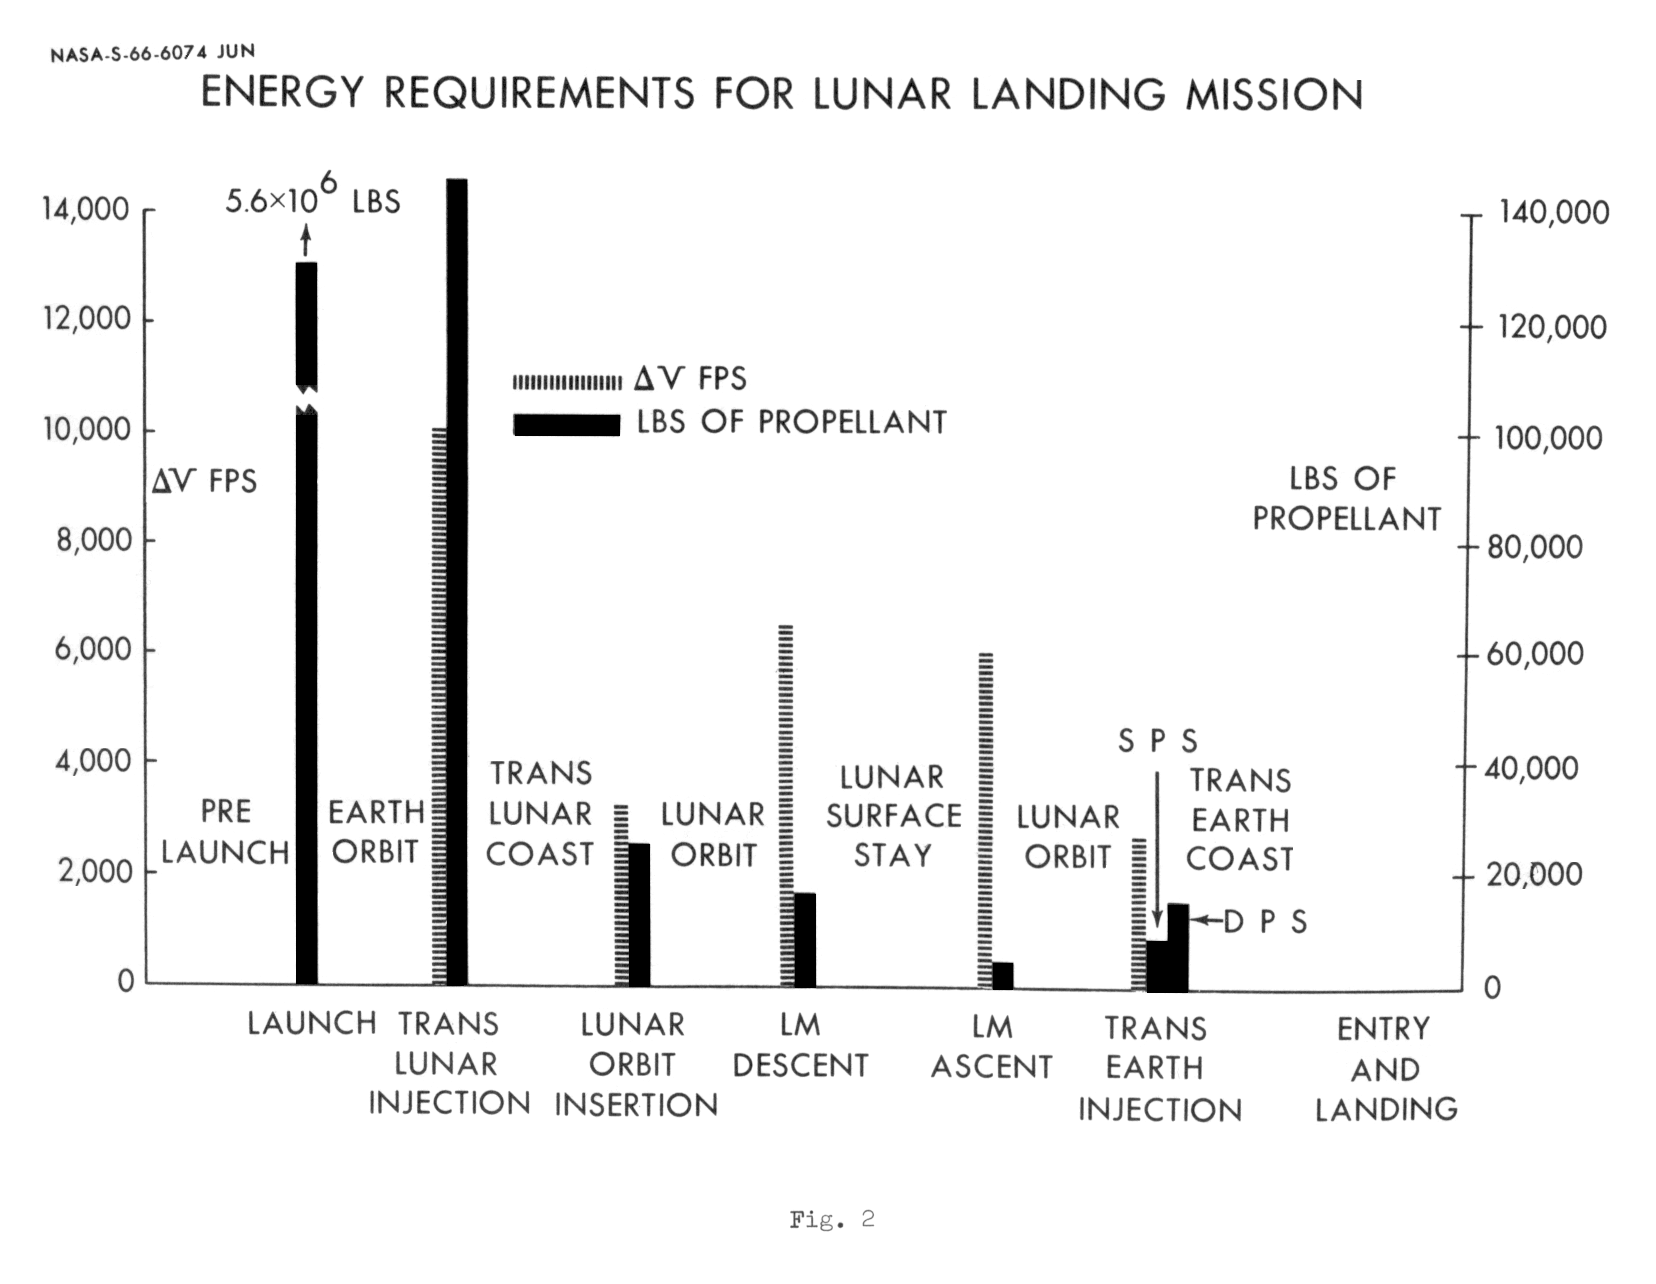
\includegraphics[width=\textwidth]{images/apollo-delta-v.png}
  \caption{Summary of energy requirements for an Apollo Lunar Landing Mission, illustrating the use of Delta-V for mission planning.\cite{maynard1966}}
  \label{fig:apollo-delta-v}
\end{figure}

\printunsrtglossary[type=symbols,style=long]

\clearpage\phantomsection
\addcontentsline{toc}{chapter}{References}
\bibliographystyle{plainnat}
\bibliography{references.bib}

\end{document}
